\chapter{绪论}

\section{课题背景}

如何使计算机能够像人类一样思考、决策、行动这是人工智能科学家长久以来一直思考的问题。\cite{AIMD} 从20世纪六十年代, 科研工作者普遍关心的是如何利用计算机解决听觉、视觉、语言理解、自动推理等问题。 但是这些问题,尤其是计算机视觉和语音识别问题, 在相当长的一段时间内发展缓慢。 这是因为, 基于之前以分析为主的方法, 例如基于边缘检测等人工主观判断的特征进行图像识别, 或者利用语言学的专家知识进行语义理解和语音识别。 自从1987年, 卡内基梅隆大学李开复博士使用统计概率模型使得当时的语言识别技术大大提升, 使得人们开始注重利用统计学习模型进行人工智能相关问题的解决。 \cite{50_years_ai} \cite{manning2008introduction} \cite{abelson1985structure}

1986年, 时任加州大学圣地亚脑科学认知实验室的研究院Geoffery Hinton在Nature杂志上发表了一种利用反向传播(Back Propagation)自动优化神经网络模型的方法, 利用神经网络进行机器学习第二次成为机器学习研究的重点。 当时确实解决了一些复杂的问题, 例如1997年YaLeCun提出的卷积神经网络(Convolutional Neural Networks)能够识别手写的阿拉伯数字, 这在计算机尤其是人工智能领域是很重要的进步。 但是, 神经网络的参数多, 为了使得其参数收敛至稳定值, 需要大量的训练样本而且其巨大的矩阵运算是一般的计算机所不能承受的, 神经网络虽然有了一些优秀的表现, 但是并没有产生突破性的表现。 

2012年ImageNet计算机视觉识别比赛中,在加拿大蒙特利尔大学担任教授的Geoffery Hinton带领团队使得ImageNet图像识别的错误率由30\%以上下降到15\%一下, 这引起了轰动。 \cite{DBLP:journals/corr/abs-1301-3781} 


\begin{figure}[htbp]
    \centering 
    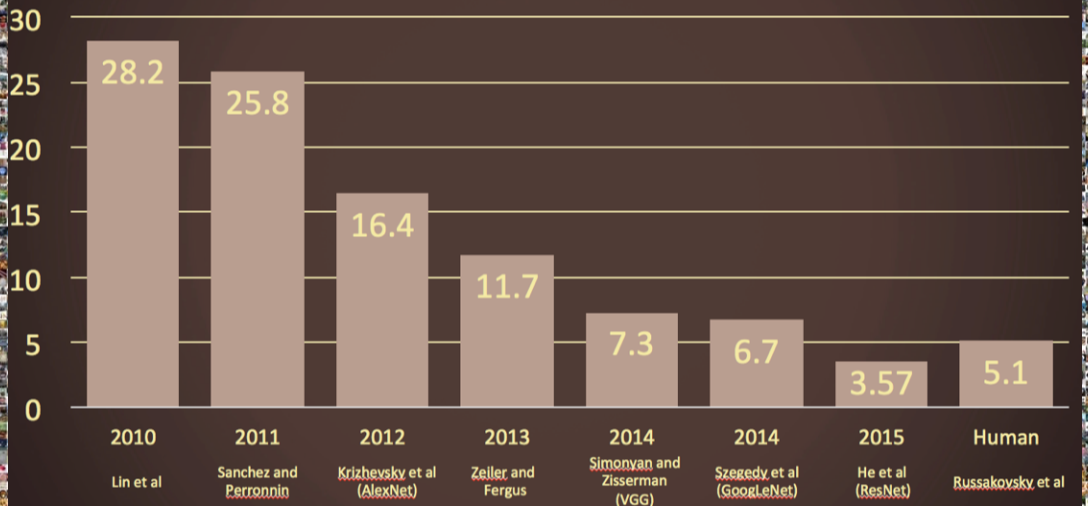
\includegraphics[width = .85\linewidth]{figures/Archive/image_net_rank.png} % 设定图片宽度相对于版心宽度,图片文件资源名
    \caption{ImageNet 错误率的下降} % 图的题注
    \label{Russakovsky et al. arXiv, 2014} 
\end{figure}


从2012年之后, 深度学习这一机器学习范式, 被用来解决诸多问题。 例如此前的ImageNet下进行的计算机视觉比赛, 在2015年其识别的错误率已经低于人类的平均值。 2017年12月22日, 腾讯DPDAC NLP实验室使用深度学习神经网络训练的自然语言理解模型, 在机器阅读理解的比赛上的正确率已经达到81.790\%, 人类在这项测试中的评价准确率为\%82.304。 除计算机视觉和自然语言理解领域, 深度学习在决策领域也表现出了惊人的进步, 2017年10月, Google Deep Mind的AlphGo战胜了战胜了围棋世界排名第一的柯洁, 这表明深度学习在复杂决策上也是具有非常大的潜力。 

由于深度学习在计算机视觉、自然语言理解、决策等方面的突出表现。 科研工作者希望利用深度学习能够解决更加类似于人类的工作, 例如 -- 艺术创作。 艺术创作长期以来被认为是人类独有的能力。 经过科学家们对于艺术创作过程以及艺术创作心理学的分析发现, 人类的艺术创作除了精神与心理学等生理原因, 其后天影响, 周围环境影响对艺术创作也是具有非常大的影响。 或者说,创意,创造力和后天学习具有密不可分的关系。 \cite{mq-zhanjian} \cite{adomavicius2005toward} \cite{gil2010state}

因此,计算机辅助艺术设计例如计算机绘画、计算机自动上色等,甚至计算机生成艺术作品在深度学习的逐渐应用的现在,被科学家们寄予希望。计算机辅助设计工具非常常见,各类基于线条信息表示的计算机图像,常常运用在设计图纸中,如建筑图纸、平面图、产品工程图、地形图、流程线框图等。基于明暗的真实感图形,也常常运用在插画、游戏、产品效果图等中,例如3d渲染、数字插图等。而从事数字绘画、动画、数字雕塑的艺术家,更是完全的通过计算机进行创作。设计师和艺术家们往往运用软件辅助进行设计和创作,软件是一个执行工具,设计师和艺术家们仍然是设计和创作的主体。

而自动生成图像的工作涉及人类的感受、逻辑、创意。对于人类自身而言,设计是探讨解决问题的方式,常常依赖于设计师敏锐的感知力、知识和经验、逻辑思维、共情能力;艺术更是人类艺术家感受、思考的结晶。对于计算机来说,一方面生成真实感图像的工作,受制于真实感图像兼顾模糊性和逻辑性,故而并不简单;另一方面生成风格化的作品也由于人类感受细腻微妙且复杂多变,人类的表达方式也非常多样化,无法拥有独属于人类的创造力。即便计算机能够将3d模型渲染出合理的光影,可是要计算机得到设计和创造的能力实在是困难之极。这一切都使自动生成图像成为一个挑战性极强的领域。而人类持续探索这一领域,也正是因为这些特点带来的魅力,机器是否也可以拥有人类的感受力、理解力、逻辑思维和创造力,这个问题正是所有计算机科学家的终极追求,使得科学家们在这一领域持续探索。 



\section{本文研究目标和内容}

作为一个设计师,在每个项目中,选取合适的配色方案是一个重要的工作。人类能够分辨某些色彩组合是和谐的而另外一些是不和谐的,某些色彩让人感觉兴奋而另一些让人感觉冷静,在色彩理论上,根据人类的生理、文化等等研究的色彩理论非常多,但是却很难讲清楚色彩和感受的关系,没有一个数学模型可以完整的解答这个答案。

设计师对作品采用某种配色都是有目的的,往往需要和环境一起为使用者带来一定的感受。比如儿童乐园的配色、玩具的配色往往鲜艳而给人带来活泼快乐的感受;医院的配色、医疗设施的配色需要给人带来温和舒适并且干净可靠的感受。我们在设计中往往首先使用语言来描述这些满足需求的感受,然后设计师会根据这些需求配色,然而自动化这一程序也同样是很困难的。人类语言描述的需求和色彩给人的感受之间的对应关系也是难以明确的。

事实上,设计色彩方案并制作色卡对于很多设计师也是有挑战性的,设计师常常需要使用线上的配色器,或者借鉴摄影作品、艺术作品等。可以说,艺术作品是设计灵感重要的产生源泉之一。如图~\ref{figure:从艺术品中借鉴色彩方案的设计作品},图中的产品设计和平面设计的配色都来自于莫奈的油画作品图~\ref{figure:从艺术品中借鉴色彩方案的设计作品}a。

\begin{figure}[!htbp]
\centering
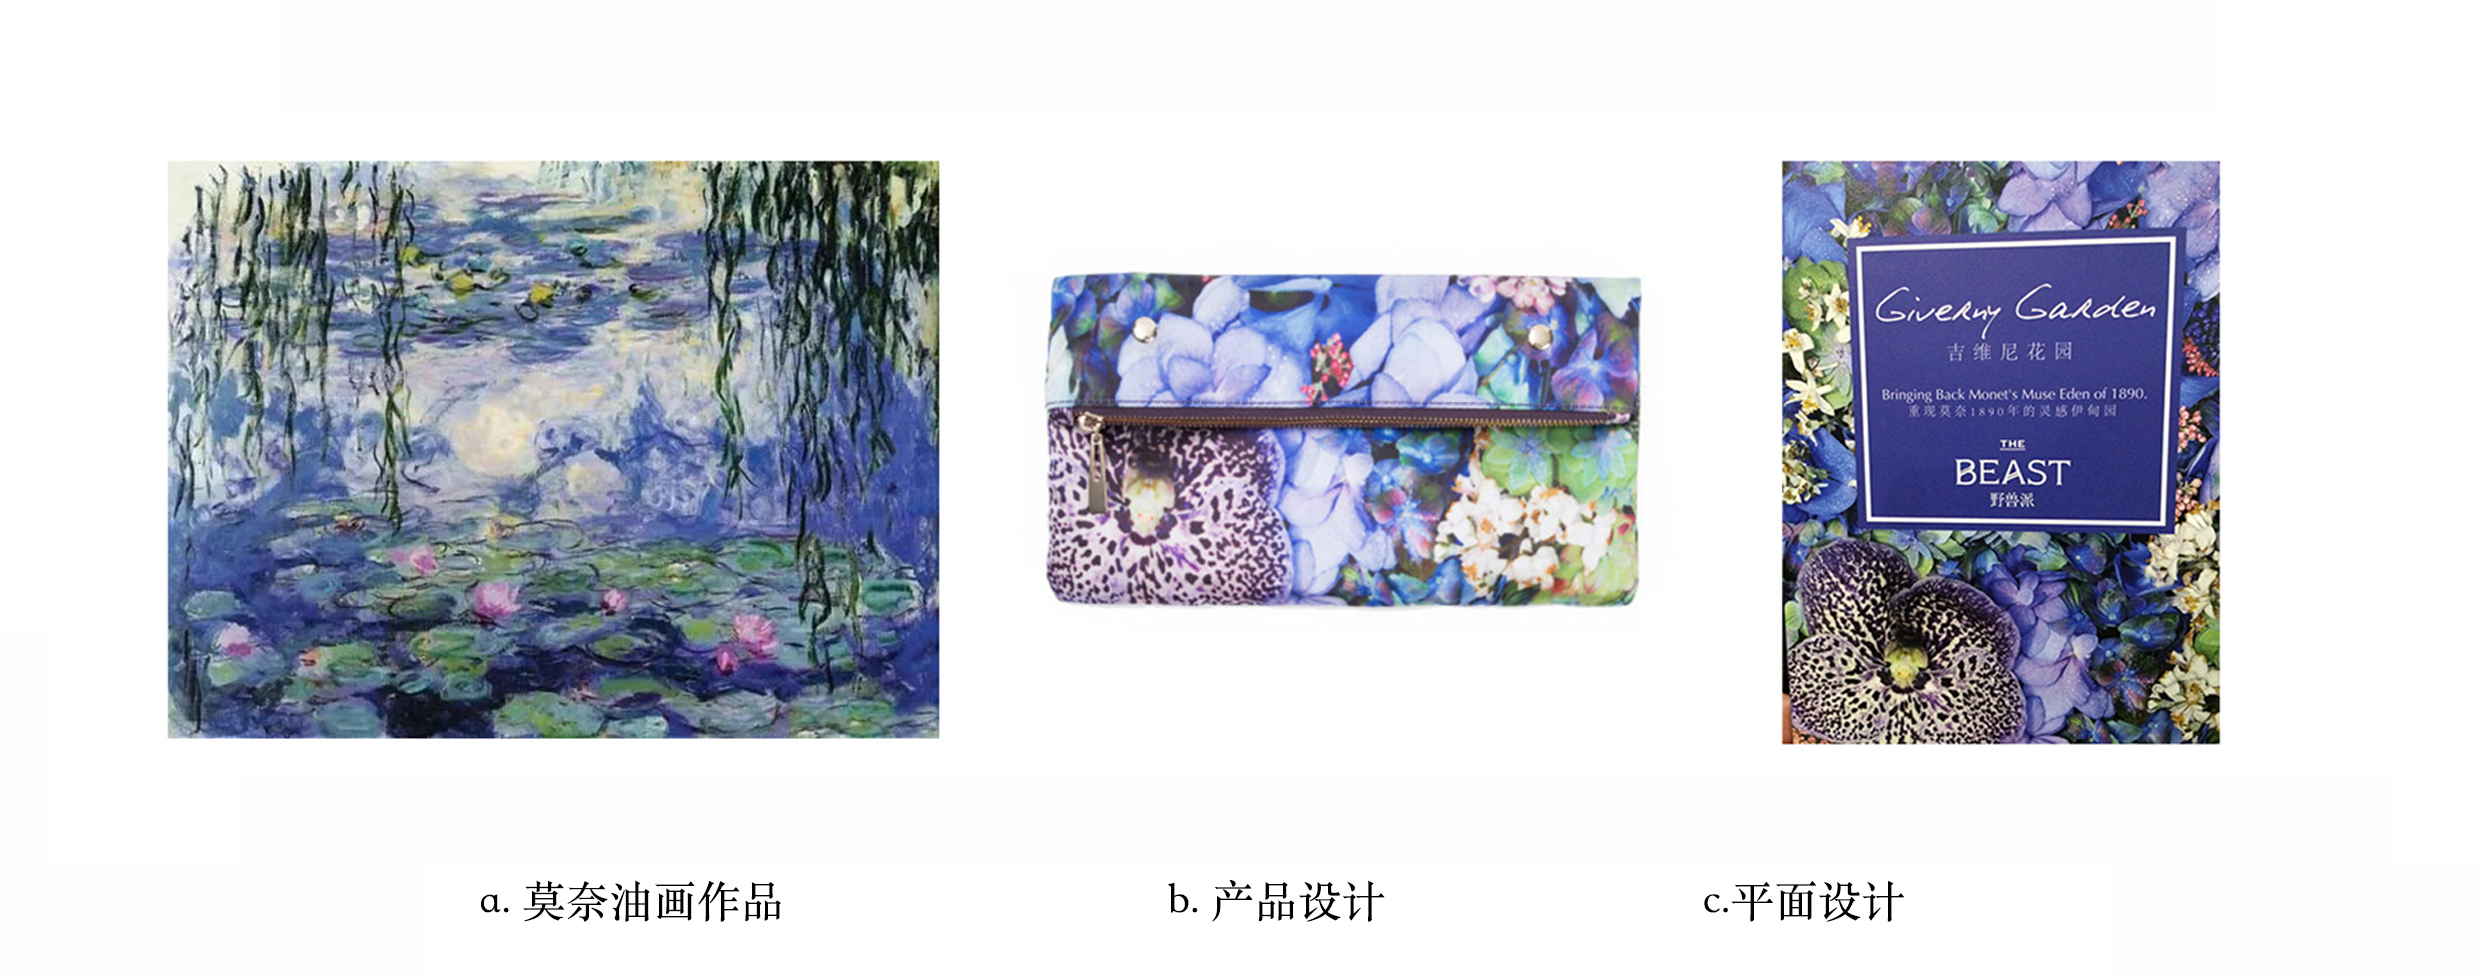
\includegraphics[width=\linewidth,keepaspectratio]{data/chapter-1/借鉴艺术品的设计.jpg}
\caption{从艺术品中借鉴色彩方案的设计作品}
\label{figure:从艺术品中借鉴色彩方案的设计作品}
\end{figure}

本文提出了一种基于语义智能理解的自动配色和上色系统。目前自动上色系统通常通过人工标注色彩、有限类型进行色彩填充或依赖已有色彩风格进行迁移,本系统通过从巨大的数据库中的艺术品学习,从艺术作品中提取色彩方案。依托艺术品图像和文本(包括介绍和题目)对应关系,使得系统直接智能地对人类的语言进行响应。实现根据文本输入来输出设计效果图的配色。

本文的实现方式如下:

1. 本系统依托艺术品交易数据库的内容进行机器学习和训练神经网络,对于数据库中的每一件艺术品有下列信息:艺术品的题目、类型、艺术品的文字描述、艺术品的图片(即绘画作品的内容),作者等。

2. 输入需求的文本描述,通过语义搜索的方式可以找出与之关联度高的艺术品文字及介绍,依托艺术品数据库中艺术品的的图像和文字介绍的匹配对应,即找出与输入文本关联度高的图片。

3. 从图片中提取色彩方案,包括绘画作品的色彩和配色比例。

4. 将提取的色彩方案运用到设计效果图上预览。上色使用泛洪填充算法(Flood Fill Algorithm)与随机游走(Random Walk)的方式,并且使用图层混合算法完成效果图的预览。

对于设计师而言,本系统可以将需求的文本描述即时转化为配色方案对设计线稿进行填充,方便的批量生成多个色彩方案以供选择,大大方便了其使用便捷性。

本文为了实现这个系统使用了三个创新点:1.使用了深度学习模型对语义进行理解;2.将图片信息与语义层面的隐藏信息进行关联,其图片风格相似性的偏序特性被保持到其语义描述的偏序特性中;3.本文使用了泛洪填充算法和随机游走的方式,对图像进行自动填充。

本文解决的难点一共有4点:1.使用word2vec对输入的文字、艺术品信息进行语义理解,设计带有语义信息的编码形式;2.输入文字编码信息与艺术品文本的编码信息对比,在数万条艺术品文本信息中搜索其中距离最近者;3.艺术品的色彩特征提取;4上色出现的一系列问题:色彩连续性、色彩比例等。

\section{本文结构安排}

本文为了实现基于语义智能理解的自动配色和上色,首先探索若干类似的课题:

之后本文详细的描述了系统的设计和实现过程。系统的整体结构从算法实现结构以及用户逻辑结构两方面设计。而系统的实现主要涉及自然语言处理,语义编码和搜索,色彩提取,上色四个方面。

最后展示该系统的的结果,通过输入语句案例进行测试,各类效果图测试案例测试该系统的理解能力、准确性、可用性、可拓展性。


